\documentclass[]{article}
\usepackage[left=1in,top=1in,right=1in,bottom=1in]{geometry}


%%%% more monte %%%%
% thispagestyle{empty}
% https://stackoverflow.com/questions/2166557/how-to-hide-the-page-number-in-latex-on-first-page-of-a-chapter
\usepackage{color}
% \usepackage[table]{xcolor} % are they using color?

% \definecolor{WSU.crimson}{HTML}{981e32}
% \definecolor{WSU.gray}{HTML}{5e6a71}

% \definecolor{shadecolor}{RGB}{248,248,248}
\definecolor{WSU.crimson}{RGB}{152,30,50} % use http://colors.mshaffer.com to convert from 981e32
\definecolor{WSU.gray}{RGB}{94,106,113}

%%%%%%%%%%%%%%%%%%%%%%%%%%%%

\newcommand*{\authorfont}{\fontfamily{phv}\selectfont}
\usepackage{lmodern}


  \usepackage[T1]{fontenc}
  \usepackage[utf8]{inputenc}




\usepackage{abstract}
\renewcommand{\abstractname}{}    % clear the title
\renewcommand{\absnamepos}{empty} % originally center

\renewenvironment{abstract}
 {{%
    \setlength{\leftmargin}{0mm}
    \setlength{\rightmargin}{\leftmargin}%
  }%
  \relax}
 {\endlist}

\makeatletter
\def\@maketitle{%
  \pagestyle{empty}
  \newpage
%  \null
%  \vskip 2em%
%  \begin{center}%
  \let \footnote \thanks
    {\fontsize{18}{20}\selectfont\raggedright  \setlength{\parindent}{0pt} \@title \par}%
}
%\fi
\makeatother






\usepackage{color}
\usepackage{fancyvrb}
\newcommand{\VerbBar}{|}
\newcommand{\VERB}{\Verb[commandchars=\\\{\}]}
\DefineVerbatimEnvironment{Highlighting}{Verbatim}{commandchars=\\\{\}}
% Add ',fontsize=\small' for more characters per line
\usepackage{framed}
\definecolor{shadecolor}{RGB}{248,248,248}
\newenvironment{Shaded}{\begin{snugshade}}{\end{snugshade}}
\newcommand{\AlertTok}[1]{\textcolor[rgb]{0.94,0.16,0.16}{#1}}
\newcommand{\AnnotationTok}[1]{\textcolor[rgb]{0.56,0.35,0.01}{\textbf{\textit{#1}}}}
\newcommand{\AttributeTok}[1]{\textcolor[rgb]{0.77,0.63,0.00}{#1}}
\newcommand{\BaseNTok}[1]{\textcolor[rgb]{0.00,0.00,0.81}{#1}}
\newcommand{\BuiltInTok}[1]{#1}
\newcommand{\CharTok}[1]{\textcolor[rgb]{0.31,0.60,0.02}{#1}}
\newcommand{\CommentTok}[1]{\textcolor[rgb]{0.56,0.35,0.01}{\textit{#1}}}
\newcommand{\CommentVarTok}[1]{\textcolor[rgb]{0.56,0.35,0.01}{\textbf{\textit{#1}}}}
\newcommand{\ConstantTok}[1]{\textcolor[rgb]{0.00,0.00,0.00}{#1}}
\newcommand{\ControlFlowTok}[1]{\textcolor[rgb]{0.13,0.29,0.53}{\textbf{#1}}}
\newcommand{\DataTypeTok}[1]{\textcolor[rgb]{0.13,0.29,0.53}{#1}}
\newcommand{\DecValTok}[1]{\textcolor[rgb]{0.00,0.00,0.81}{#1}}
\newcommand{\DocumentationTok}[1]{\textcolor[rgb]{0.56,0.35,0.01}{\textbf{\textit{#1}}}}
\newcommand{\ErrorTok}[1]{\textcolor[rgb]{0.64,0.00,0.00}{\textbf{#1}}}
\newcommand{\ExtensionTok}[1]{#1}
\newcommand{\FloatTok}[1]{\textcolor[rgb]{0.00,0.00,0.81}{#1}}
\newcommand{\FunctionTok}[1]{\textcolor[rgb]{0.00,0.00,0.00}{#1}}
\newcommand{\ImportTok}[1]{#1}
\newcommand{\InformationTok}[1]{\textcolor[rgb]{0.56,0.35,0.01}{\textbf{\textit{#1}}}}
\newcommand{\KeywordTok}[1]{\textcolor[rgb]{0.13,0.29,0.53}{\textbf{#1}}}
\newcommand{\NormalTok}[1]{#1}
\newcommand{\OperatorTok}[1]{\textcolor[rgb]{0.81,0.36,0.00}{\textbf{#1}}}
\newcommand{\OtherTok}[1]{\textcolor[rgb]{0.56,0.35,0.01}{#1}}
\newcommand{\PreprocessorTok}[1]{\textcolor[rgb]{0.56,0.35,0.01}{\textit{#1}}}
\newcommand{\RegionMarkerTok}[1]{#1}
\newcommand{\SpecialCharTok}[1]{\textcolor[rgb]{0.00,0.00,0.00}{#1}}
\newcommand{\SpecialStringTok}[1]{\textcolor[rgb]{0.31,0.60,0.02}{#1}}
\newcommand{\StringTok}[1]{\textcolor[rgb]{0.31,0.60,0.02}{#1}}
\newcommand{\VariableTok}[1]{\textcolor[rgb]{0.00,0.00,0.00}{#1}}
\newcommand{\VerbatimStringTok}[1]{\textcolor[rgb]{0.31,0.60,0.02}{#1}}
\newcommand{\WarningTok}[1]{\textcolor[rgb]{0.56,0.35,0.01}{\textbf{\textit{#1}}}}



\title{\textbf{\textcolor{WSU.crimson}{Height and Body Proportions of Different Ethnicities}}  }

%  

% \author{ \Large true \hfill \normalsize \emph{} }
\author{\Large Connor StarrHurst\vspace{0.05in} \newline\normalsize\emph{Washington State University}  }


\date{November 11, 2020}
\setcounter{secnumdepth}{3}

\usepackage{titlesec}
% See the link above: KOMA classes are not compatible with titlesec any more. Sorry.
% https://github.com/jbezos/titlesec/issues/11
\titleformat*{\section}{\bfseries}
\titleformat*{\subsection}{\bfseries\itshape}
\titleformat*{\subsubsection}{\itshape}
\titleformat*{\paragraph}{\itshape}
\titleformat*{\subparagraph}{\itshape}

% https://code.usgs.gov/usgs/norock/irvine_k/ip-092225/


%\titleformat*{\section}{\normalsize\bfseries}
%\titleformat*{\subsection}{\normalsize\itshape}
%\titleformat*{\subsubsection}{\normalsize\itshape}
%\titleformat*{\paragraph}{\normalsize\itshape}
%\titleformat*{\subparagraph}{\normalsize\itshape}

% https://tex.stackexchange.com/questions/233866/one-column-multicol-environment#233904
\usepackage{environ}
\NewEnviron{auxmulticols}[1]{%
  \ifnum#1<2\relax% Fewer than 2 columns
    %\vspace{-\baselineskip}% Possible vertical correction
    \BODY
  \else% More than 1 column
    \begin{multicols}{#1}
      \BODY
    \end{multicols}%
  \fi
}





\usepackage{natbib}
\setcitestyle{aysep={}} %% no year, comma just year
% \usepackage[numbers]{natbib}
\bibliographystyle{./../biblio/ormsv080.bst}



\usepackage[strings]{underscore} % protect underscores in most circumstances




\newtheorem{hypothesis}{Hypothesis}
\usepackage{setspace}


%%%%%%%%%%%%%%%%%%%%%%%%%%%%%%%%%%%%%%%%%%%%%%%%%%%%%
%%% MONTE ADDS %%%

\usepackage{fancyhdr} % fancy header 
\usepackage{lastpage} % last page 

\usepackage{multicol}


\usepackage{etoolbox}
\AtBeginEnvironment{quote}{\singlespacing\small}
% https://tex.stackexchange.com/questions/325695/how-to-style-blockquote


\usepackage{soul}			%% allows strike-through
\usepackage{url}			%% fixes underscores in urls
\usepackage{csquotes}		%% allows \textquote in references
\usepackage{rotating}		%% allows table and box rotation
\usepackage{caption}		%% customize caption information
\usepackage{booktabs}		%% enhance table/tabular environment
\usepackage{tabularx}		%% width attributes updates tabular
\usepackage{enumerate}		%% special item environment
\usepackage{enumitem}		%% special item environment

\usepackage{lineno}		%% allows linenumbers for editing using \linenumbers
\usepackage{hanging}


\usepackage{mathtools}  	%% also loads amsmath
\usepackage{bm}		%% bold-math
\usepackage{scalerel}	%% scale one element (make one beta bigger font)

\newcommand{\gFrac}[2]{ \genfrac{}{}{0pt}{1}{{#1}}{#2} }

\newcommand{\betaSH}[3]{  \gFrac{\text{\tiny #1}}{{\text{\tiny #2}}}\hat{\beta}_{\text{#3}}   }
\newcommand{\betaSB}[3]{              ^{\text{#1}} _{\text{#2}} \bm{\beta} _{\text{#3}}                   }  %% bold
\newcommand{\bigEQ}{  \scaleobj{1.5}{{\ }= } }
\newcommand{\bigP}[1]{  \scaleobj{1.5}{#1 } }





\usepackage{endnotes}  % he already does this ...
\renewcommand{\enotesize}{\normalsize}
% https://tex.stackexchange.com/questions/99984/endnotes-do-not-be-superscript-and-add-a-space
\renewcommand\makeenmark{\textsuperscript{[\theenmark]}} % in brackets %
% https://tex.stackexchange.com/questions/31574/how-to-control-the-indent-in-endnotes
\patchcmd{\enoteformat}{1.8em}{0pt}{}{}

\patchcmd{\theendnotes}
  {\makeatletter}
  {\makeatletter\renewcommand\makeenmark{\textbf{[\theenmark]} }}
  {}{}



% https://tex.stackexchange.com/questions/141906/configuring-footnote-position-and-spacing

\addtolength{\footnotesep}{5mm} % change to 1mm

\renewcommand{\thefootnote}{\textbf{\arabic{footnote}}}
\let\footnote=\endnote
%\renewcommand*{\theendnote}{\alph{endnote}}
%\renewcommand{\theendnote}{\textbf{\arabic{endnote}}}


\renewcommand*{\notesname}{ENDNOTES}

\makeatletter
\def\enoteheading{\section*{\notesname
  \@mkboth{\MakeUppercase{\notesname}}{\MakeUppercase{\notesname}}}%
  \mbox{}\par\vskip-2.3\baselineskip\noindent\rule{.5\textwidth}{0.4pt}\par\vskip\baselineskip}
\makeatother


\renewcommand*{\contentsname}{TABLE OF CONTENTS}

\renewcommand*{\refname}{REFERENCES}


%\usepackage{subfigure}
\usepackage{subcaption}

\captionsetup{labelfont=bf}  % Make Table / Figure bold

%%% you could add elements here ... monte says .... %%%
%\usepackage{mypackageForCapitalH}


%%%%%%%%%%%%%%%%%%%%%%%%%%%%%%%%%%%%%%%%%%%%%%%%%%%%%

% set default figure placement to htbp
\makeatletter
\def\fps@figure{htbp}
\makeatother


% move the hyperref stuff down here, after header-includes, to allow for - \usepackage{hyperref}

\makeatletter
\@ifpackageloaded{hyperref}{}{%
\ifxetex
  \PassOptionsToPackage{hyphens}{url}\usepackage[setpagesize=false, % page size defined by xetex
              unicode=false, % unicode breaks when used with xetex
              xetex]{hyperref}
\else
  \PassOptionsToPackage{hyphens}{url}\usepackage[draft,unicode=true]{hyperref}
\fi
}

\@ifpackageloaded{color}{
    \PassOptionsToPackage{usenames,dvipsnames}{color}
}{%
    \usepackage[usenames,dvipsnames]{color}
}
\makeatother
\hypersetup{breaklinks=true,
            bookmarks=true,
            pdfauthor={Connor StarrHurst (Washington State University)},
             pdfkeywords = {multiple comparisons to control; body measurements; body proportions;
IQR; descriptive statistics; correlation analysis;},  
            pdftitle={Height and Body Proportions of Different Ethnicities},
            colorlinks=true,
            citecolor=blue,
            urlcolor=blue,
            linkcolor=magenta,
            pdfborder={0 0 0}}
\urlstyle{same}  % don't use monospace font for urls

% Add an option for endnotes. -----

%
% add tightlist ----------
\providecommand{\tightlist}{%
\setlength{\itemsep}{0pt}\setlength{\parskip}{0pt}}

% add some other packages ----------

% \usepackage{multicol}
% This should regulate where figures float
% See: https://tex.stackexchange.com/questions/2275/keeping-tables-figures-close-to-where-they-are-mentioned
\usepackage[section]{placeins}



\pagestyle{fancy}   
\lhead{\textcolor{WSU.crimson}{\textbf{ Height and Body Proportions of Different Ethnicities }}}
\chead{}
\rhead{\textcolor{WSU.gray}{\textbf{  Page\ \thepage\ of\ \protect\pageref{LastPage} }}}
\lfoot{}
\cfoot{}
\rfoot{}


\begin{document}
	
% \pagenumbering{arabic}% resets `page` counter to 1 
%
% \maketitle

{% \usefont{T1}{pnc}{m}{n}
\setlength{\parindent}{0pt}
\thispagestyle{plain}
{\fontsize{18}{20}\selectfont\raggedright 
\maketitle  % title \par  

}

{
   \vskip 13.5pt\relax \normalsize\fontsize{11}{12} 
   
\textbf{\authorfont Connor StarrHurst} \hskip 15pt \emph{\small Washington State University}   

}

}








\begin{abstract}

    \hbox{\vrule height .2pt width 39.14pc}

    \vskip 8.5pt % \small 

\noindent In this article, we compare the body measurements of 251 people from
various ethnic backgrounds. We first hypothesized that European and
American ethnicities (White, Caucasian, Anglo) are typically taller than
Asian ethnicities (Asian, Chinese, Korean, Japanese) and concluded that
European and American ethnicities are typically taller than Asian
ethnicities. We then hypothesized that European and American ethnicities
(White, Caucasian, Anglo) are typically shorter than Hispanic and Latin
American ethnicities (Hispanic, Latin American, Asian-Latino) and
concluded that European and American ethnicities are not typically
shorter than Latin American ethnicities. \vspace{0.25in}


\vskip 8.5pt \noindent \textbf{\underline{Keywords}:} multiple comparisons to control; body measurements; body proportions;
IQR; descriptive statistics; correlation analysis; \par

    




    
    \hbox{\vrule height .2pt width 39.14pc}
    \vskip 5pt 
    \hfill \textbf{\textcolor{WSU.gray}{ November 11, 2020 } }
    \vskip 5pt 
    
\end{abstract}


\vskip -8.5pt



 % removetitleabstract

\noindent  

\section{Introduction}
\label{sec:intro}

\begin{figure}[!ht]
%OnePlot
    \hrule
    \caption{ \textbf{Comparision of Height and Head Proportions per Ethnicity} }
    \begin{center}
        \scalebox{1.00}{    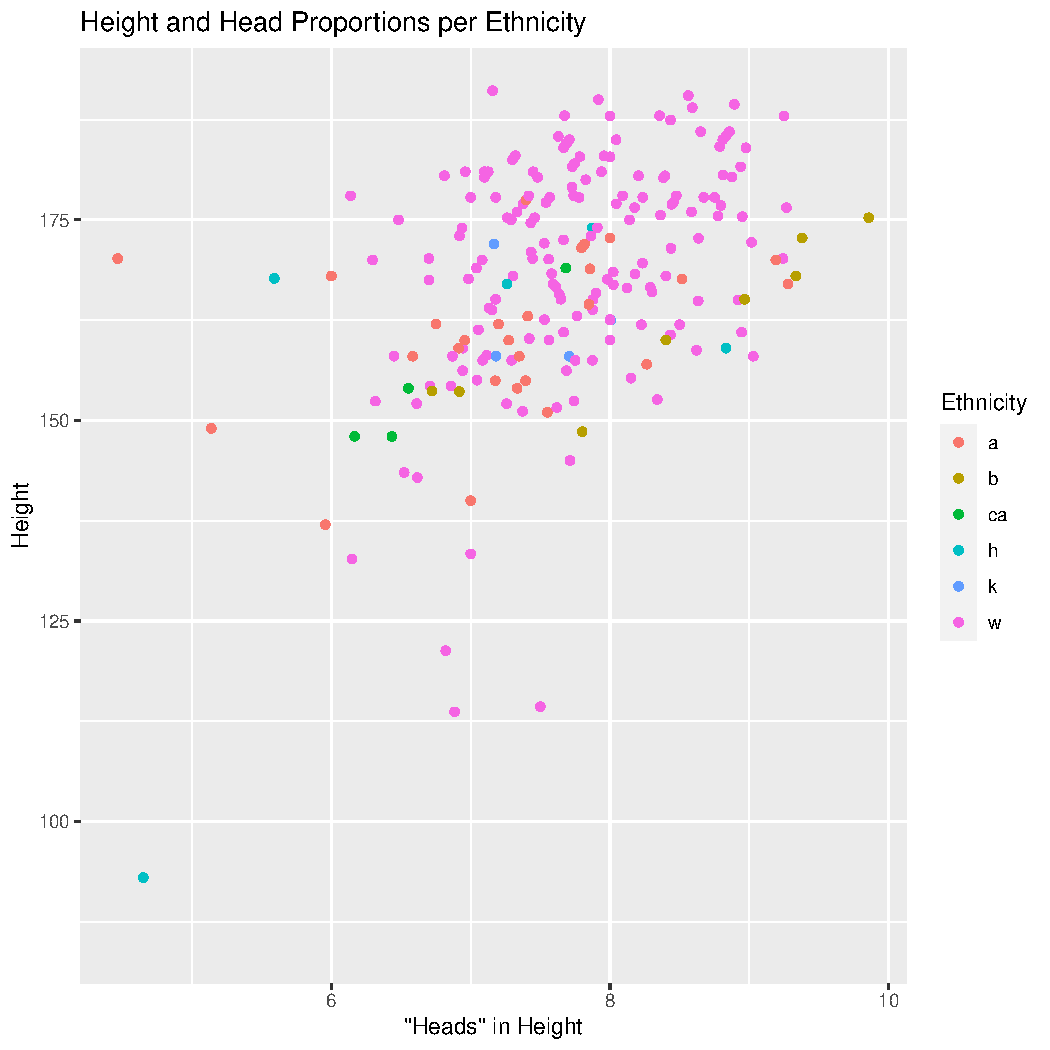
\includegraphics[trim = 0 0 0 0,clip,width=\textwidth]{tables/OnePlot.pdf} }
    \end{center}
    \label{fig:OnePlot}
    \hrule
\end{figure}

\newpage

\begin{figure}[!ht]
%TwoPlot
    \hrule
    \caption{ \textbf{IQR of Height per Ethnicity} }
    \begin{center}
        \scalebox{1.00}{    \includegraphics[trim = 0 0 0 0,clip,width=\textwidth]{tables/TwoPlot.pdf} }
    \end{center}
    \label{fig:TwoPlot}
    \hrule
\end{figure}

\newpage

a = Asian, b = African American, ca = Caucasian/Asian, h = Hispanic, k =
Korean, w = White

\section{Research Question:  Do certain ethnicities have specific body proportions?}
\label{sec:rq}

\subsection{Are White, Caucasian, and Anglo ethnicities generally taller than Asian, Chinese, Japanese, and Korean ethnicities?}
\label{sec:rq2}

\subsection{Are White, Caucasian, and Anglo ethnicities generally shorter than Hispanic, Latin American, and Asian-Latino ethnicities?}
\label{sec:rq3}

\section{Data Description}
\label{sec:data}

\subsection{Summary Statistics of Data}
\label{sec:data-summary}

\begin{sidewaystable}[!htbp]
\footnotesize
\centering
\caption{\textbf{Descriptive Statistics and Correlation Analysis}}
\label{table:correlation}
\begin{tabularx}{0.975\textwidth}{{r@{ \ \ } p{35mm} r@{}lp{.25mm} r@{}l p{.5mm} r@{}l p{.01mm} r@{}l p{.01mm} r@{}l p{.01mm} r@{}l p{.01mm} r@{}l p{.01mm} r@{}l p{.01mm} r@{}l p{.01mm} r@{}l p{.01mm} r@{}l p{.01mm} r@{}l p{.01mm} r@{}l p{.01mm}   r@{}l  }}
 & \\
\hline
 & \\
\multicolumn{2}{c}{\textbf{ }} & \multicolumn{2}{c}{\textbf{M}} & & \multicolumn{2}{c}{\textbf{SD}} &  & \multicolumn{2}{c}{\textbf{1}} &  & \multicolumn{2}{c}{\textbf{2}} &  & \multicolumn{2}{c}{\textbf{3}} &  & \multicolumn{2}{c}{\textbf{4}} &  & \multicolumn{2}{c}{\textbf{5}} &  & \multicolumn{2}{c}{\textbf{6}} &  & \multicolumn{2}{c}{\textbf{7}} &  & \multicolumn{2}{c}{\textbf{8}} &  & \multicolumn{2}{c}{\textbf{9}} &  & \multicolumn{2}{c}{\textbf{10}} &  & \multicolumn{2}{c}{\textbf{11}} &  & \\ 
 & \\
\hline
 & \\
\textbf{1} & \textbf{Height (cm)} &  167&.3 &  &  15&.24 &  &  \multicolumn{2}{c}{1}  &  &  \multicolumn{2}{c}{ \  \  \  \  \ }  &  &  \multicolumn{2}{c}{ \  \  \  \  \ }  &  &  \multicolumn{2}{c}{ \  \  \  \  \ }  &  &  \multicolumn{2}{c}{ \  \  \  \  \ }  &  &  \multicolumn{2}{c}{ \  \  \  \  \ }  &  &  \multicolumn{2}{c}{ \  \  \  \  \ }  &  &  \multicolumn{2}{c}{ \  \  \  \  \ }  &  &  \multicolumn{2}{c}{ \  \  \  \  \ }  &  &  \multicolumn{2}{c}{ \  \  \  \  \ }  &  &  \multicolumn{2}{c}{ \  \  \  \  \ }  &  & \\ 
 & \\
\textbf{2} & \textbf{Arm Span (cm)} &  167&.4 &  &  21&.54 &  &  &.72{$^{***}$}  &  &  \multicolumn{2}{c}{1}  &  &  \multicolumn{2}{c}{ \  \  \  \  \ }  &  &  \multicolumn{2}{c}{ \  \  \  \  \ }  &  &  \multicolumn{2}{c}{ \  \  \  \  \ }  &  &  \multicolumn{2}{c}{ \  \  \  \  \ }  &  &  \multicolumn{2}{c}{ \  \  \  \  \ }  &  &  \multicolumn{2}{c}{ \  \  \  \  \ }  &  &  \multicolumn{2}{c}{ \  \  \  \  \ }  &  &  \multicolumn{2}{c}{ \  \  \  \  \ }  &  &  \multicolumn{2}{c}{ \  \  \  \  \ }  &  & \\ 
 & \\
\textbf{3} & \textbf{Hand Length (cm)} &  19&.6 &  &  16&.82 &  &  &.15{$^{*}$}  &  &  &.11{$^{\dagger}$}  &  &  \multicolumn{2}{c}{1}  &  &  \multicolumn{2}{c}{ \  \  \  \  \ }  &  &  \multicolumn{2}{c}{ \  \  \  \  \ }  &  &  \multicolumn{2}{c}{ \  \  \  \  \ }  &  &  \multicolumn{2}{c}{ \  \  \  \  \ }  &  &  \multicolumn{2}{c}{ \  \  \  \  \ }  &  &  \multicolumn{2}{c}{ \  \  \  \  \ }  &  &  \multicolumn{2}{c}{ \  \  \  \  \ }  &  &  \multicolumn{2}{c}{ \  \  \  \  \ }  &  & \\ 
 & \\
\textbf{4} & \textbf{Hand to Elbow (cm)} &  42&.5 &  &  4&.60 &  &  &.70{$^{***}$}  &  &  &.60{$^{***}$}  &  &  &.10 &  &  \multicolumn{2}{c}{1}  &  &  \multicolumn{2}{c}{ \  \  \  \  \ }  &  &  \multicolumn{2}{c}{ \  \  \  \  \ }  &  &  \multicolumn{2}{c}{ \  \  \  \  \ }  &  &  \multicolumn{2}{c}{ \  \  \  \  \ }  &  &  \multicolumn{2}{c}{ \  \  \  \  \ }  &  &  \multicolumn{2}{c}{ \  \  \  \  \ }  &  &  \multicolumn{2}{c}{ \  \  \  \  \ }  &  & \\ 
 & \\
\textbf{5} & \textbf{Elbow to Armpit (cm)} &  26&.7 &  &  6&.47 &  &  &.39{$^{***}$}  &  &  &.27{$^{***}$}  &  &  &.05 &  &  &.42{$^{***}$}  &  &  \multicolumn{2}{c}{1}  &  &  \multicolumn{2}{c}{ \  \  \  \  \ }  &  &  \multicolumn{2}{c}{ \  \  \  \  \ }  &  &  \multicolumn{2}{c}{ \  \  \  \  \ }  &  &  \multicolumn{2}{c}{ \  \  \  \  \ }  &  &  \multicolumn{2}{c}{ \  \  \  \  \ }  &  &  \multicolumn{2}{c}{ \  \  \  \  \ }  &  & \\ 
 & \\
\textbf{6} & \textbf{Floor to Kneepit (cm)} &  191&.6 &  &  49&.68 &  &  &.28{$^{***}$}  &  &  &.27{$^{***}$}  &  &  &.08 &  &  &.09 &  &  -&.03 &  &  \multicolumn{2}{c}{1}  &  &  \multicolumn{2}{c}{ \  \  \  \  \ }  &  &  \multicolumn{2}{c}{ \  \  \  \  \ }  &  &  \multicolumn{2}{c}{ \  \  \  \  \ }  &  &  \multicolumn{2}{c}{ \  \  \  \  \ }  &  &  \multicolumn{2}{c}{ \  \  \  \  \ }  &  & \\ 
 & \\
\textbf{7} & \textbf{Floor to Hip (cm)} &  24&.8 &  &  2&.69 &  &  &.71{$^{***}$}  &  &  &.60{$^{***}$}  &  &  &.08 &  &  &.58{$^{***}$}  &  &  &.29{$^{***}$}  &  &  &.30{$^{***}$}  &  &  \multicolumn{2}{c}{1}  &  &  \multicolumn{2}{c}{ \  \  \  \  \ }  &  &  \multicolumn{2}{c}{ \  \  \  \  \ }  &  &  \multicolumn{2}{c}{ \  \  \  \  \ }  &  &  \multicolumn{2}{c}{ \  \  \  \  \ }  &  & \\ 
 & \\
\textbf{8} & \textbf{Floor to Armpit (cm)} &  45&.2 &  &  5&.24 &  &  &.70{$^{***}$}  &  &  &.43{$^{***}$}  &  &  &.10 &  &  &.53{$^{***}$}  &  &  &.32{$^{***}$}  &  &  &.17{$^{*}$}  &  &  &.52{$^{***}$}  &  &  \multicolumn{2}{c}{1}  &  &  \multicolumn{2}{c}{ \  \  \  \  \ }  &  &  \multicolumn{2}{c}{ \  \  \  \  \ }  &  &  \multicolumn{2}{c}{ \  \  \  \  \ }  &  & \\ 
 & \\
\textbf{9} & \textbf{NA} &  95&.3 &  &  9&.51 &  &  &.71{$^{***}$}  &  &  &.50{$^{***}$}  &  &  &.10 &  &  &.53{$^{***}$}  &  &  &.27{$^{***}$}  &  &  &.26{$^{***}$}  &  &  &.56{$^{***}$}  &  &  &.54{$^{***}$}  &  &  \multicolumn{2}{c}{1}  &  &  \multicolumn{2}{c}{ \  \  \  \  \ }  &  &  \multicolumn{2}{c}{ \  \  \  \  \ }  &  & \\ 
 & \\
\textbf{10} & \textbf{NA} &  131&.3 &  &  11&.90 &  &  &.88{$^{***}$}  &  &  &.57{$^{***}$}  &  &  &.14{$^{*}$}  &  &  &.68{$^{***}$}  &  &  &.37{$^{***}$}  &  &  &.31{$^{***}$}  &  &  &.66{$^{***}$}  &  &  &.63{$^{***}$}  &  &  &.77{$^{***}$}  &  &  \multicolumn{2}{c}{1}  &  &  \multicolumn{2}{c}{ \  \  \  \  \ }  &  & \\ 
 & \\
\textbf{11} & \textbf{NA} &  7&.6 &  &  &.87 &  &  &.43{$^{***}$}  &  &  &.40{$^{***}$}  &  &  &.13{$^{*}$}  &  &  &.29{$^{***}$}  &  &  &.22{$^{***}$}  &  &  &.12{$^{\dagger}$}  &  &  &.22{$^{***}$}  &  &  &.21{$^{**}$}  &  &  &.28{$^{***}$}  &  &  &.34{$^{***}$}  &  &  \multicolumn{2}{c}{1}  &  & \\ 
 & \\
\textbf{12} & \textbf{NA} &  50&.5 &  &  9&.61 &  &  &.65{$^{***}$}  &  &  &.45{$^{***}$}  &  &  &.11 &  &  &.41{$^{***}$}  &  &  &.26{$^{***}$}  &  &  &.21{$^{**}$}  &  &  &.38{$^{***}$}  &  &  &.38{$^{***}$}  &  &  -&.04 &  &  &.43{$^{***}$}  &  &  &.56{$^{***}$}  &  & \\ 
 & \\
\hline
 & \\
\multicolumn{40}{p{0.88\textwidth}}{  \footnotesize { \begin{hangparas}{0.75in}{1} \textbf{\underline{Notes}:} \ \ Pearson pairwise correlations are reported; \newline a two-side test was 
  performed to report correlation significance.  \end{hangparas} } }  & \\  
\multicolumn{40}{p{0.88\textwidth}}{  {\tiny {$^{\dagger} p < .10$} }  {     } {\tiny        {$^{*} p < .05$} }  {     } {\tiny       {$^{**} p < .01$} }  {     } {\tiny      {$^{***} p < .001$} } {     }     } & \\ 
 & \\
\hline
\end{tabularx}
\end{sidewaystable}


\section{Key Findings}
\label{sec:findings}

\section{Conclusion}
\label{sec:conclusion}

\section{APPENDICES}
\label{sec:appendix}

\subsection{Data Provenance}
\label{sec:appendix-data-provenance}

\subsubsection{Data Collection Handout}
\label{sec:appendix-data-handout}

\begin{figure}[!ht]
    \hrule
    \caption{ \textbf{Handout Page 1} }
    \begin{center}
        \scalebox{1.00}{    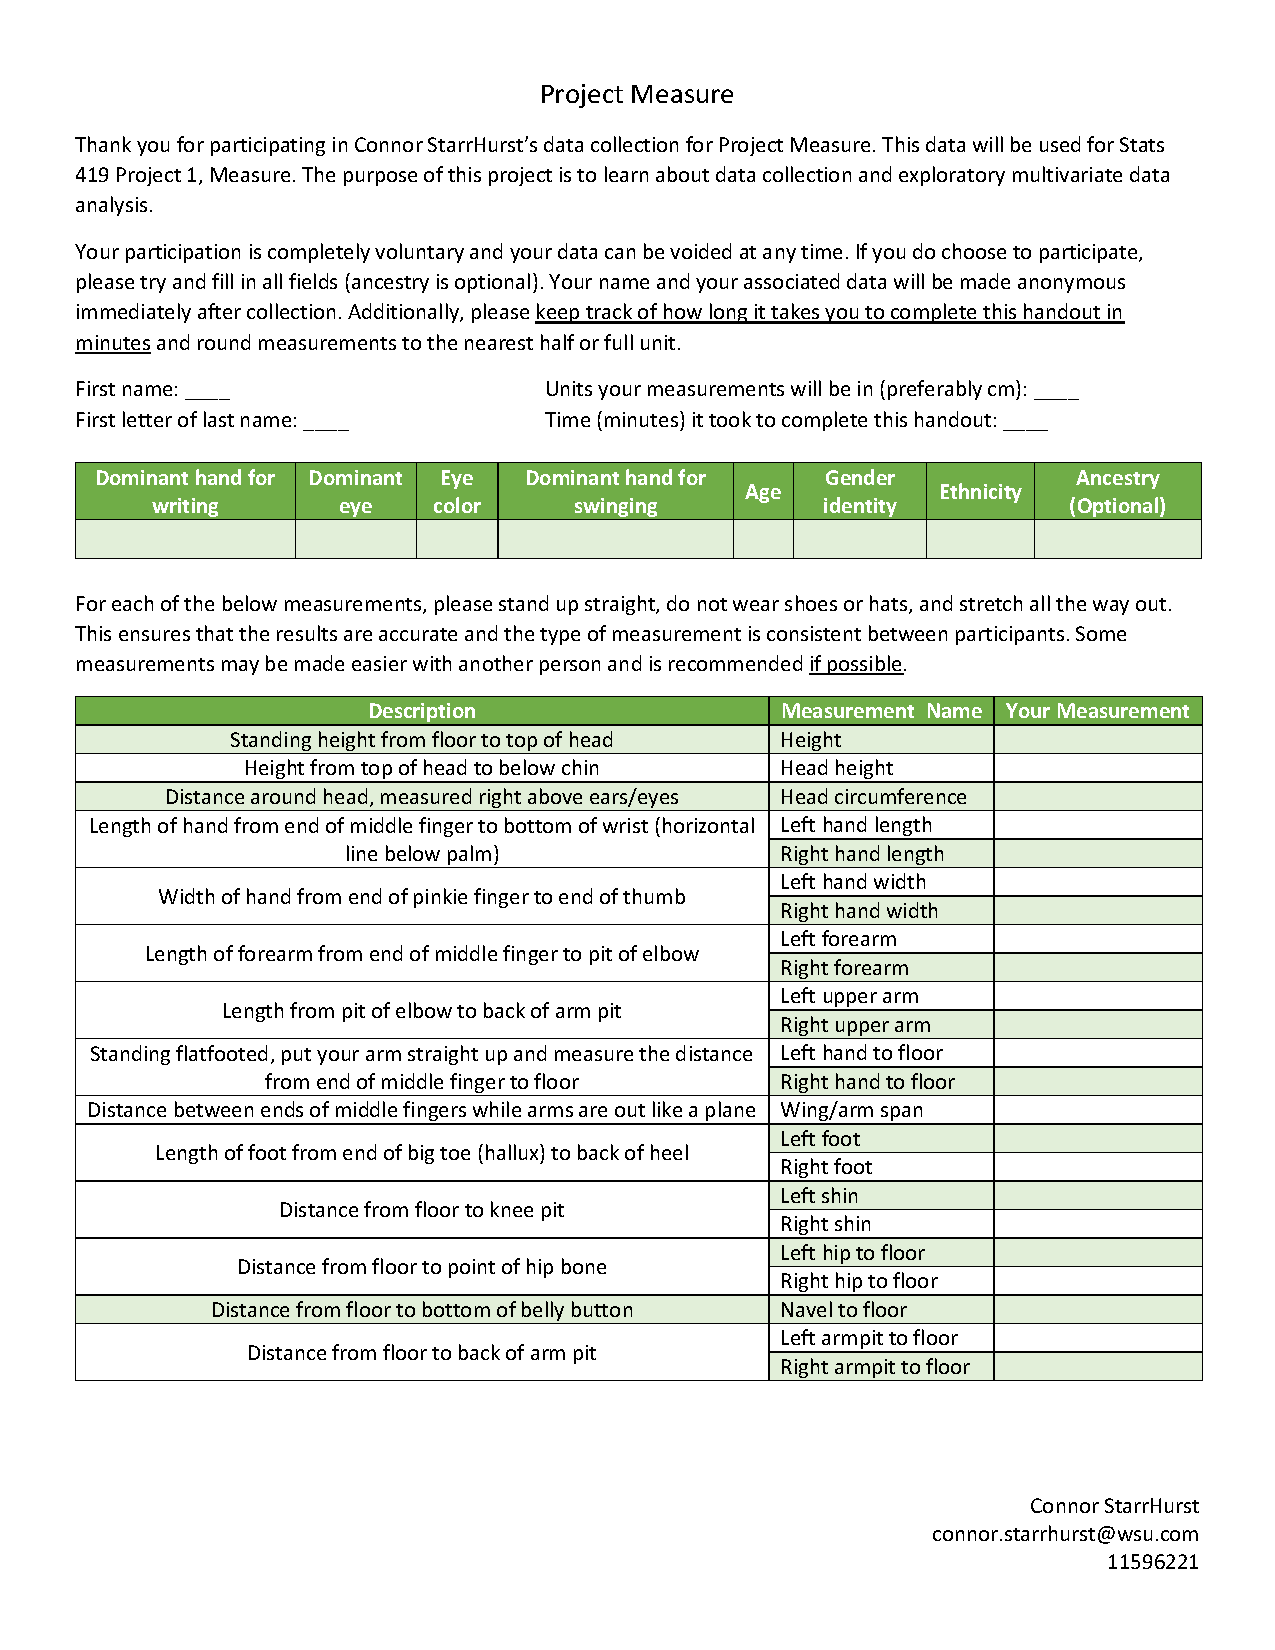
\includegraphics[trim = 0 0 0 0,clip,width=0.85\textwidth]{pdfs/Handout.pdf} }
    \end{center}
    \label{fig:handout-1}
    \hrule
\end{figure}

\newpage

\subsection{Coding the Report}
\label{sec:appendix-setup}

\subsubsection{Preparing the Data}
\label{sec:appendix-setup2}

Below is the necessary functions and libraries required to run the code
referenced in this document.

\begin{Shaded}
\begin{Highlighting}[]
\KeywordTok{library}\NormalTok{(devtools); }\CommentTok{# required for source_url}

\NormalTok{path.humanVerseWSU =}\StringTok{ "https://raw.githubusercontent.com/MonteShaffer/humanVerseWSU/"}
\KeywordTok{source_url}\NormalTok{( }\KeywordTok{paste0}\NormalTok{(path.humanVerseWSU,}\StringTok{"master/misc/functions-project-measure.R"}\NormalTok{) );}
\end{Highlighting}
\end{Shaded}

Below is the code to load the data and prepare it for analysis.

\begin{Shaded}
\begin{Highlighting}[]
\NormalTok{path.to.project =}\StringTok{ "C:/Users/Connor/.ssh/stats419/project-measure/"}\NormalTok{;}
\NormalTok{path.to.secret =}\StringTok{ }
\StringTok{  "C:/Users/Connor/Documents/1) WSU 2018-/Fall 2020/Stat 419/Project 1 Measure/"}\NormalTok{;}
\NormalTok{path.to.tables =}\StringTok{ }\KeywordTok{paste0}\NormalTok{(path.to.project,}\StringTok{"tables/"}\NormalTok{);}
  \KeywordTok{createDirRecursive}\NormalTok{(path.to.tables);}

\NormalTok{measure =}\StringTok{ }\NormalTok{utils}\OperatorTok{::}\KeywordTok{read.csv}\NormalTok{( }\KeywordTok{paste0}\NormalTok{(path.to.secret, }\StringTok{"cm.final.measure.txt"}\NormalTok{), }\DataTypeTok{header=}\OtherTok{TRUE}\NormalTok{, }
                          \DataTypeTok{quote=}\StringTok{""}\NormalTok{, }\DataTypeTok{sep=}\StringTok{"|"}\NormalTok{);}

\NormalTok{path.github =}\StringTok{ "https://raw.githubusercontent.com/youknowwwho/stats419/"}\NormalTok{;}
\KeywordTok{source_url}\NormalTok{( }\KeywordTok{paste0}\NormalTok{(path.github,}\StringTok{"master/Functions/functions-project-measure.R"}\NormalTok{) );}

\KeywordTok{set.seed}\NormalTok{(}\DecValTok{11906189}\NormalTok{);}

\NormalTok{measure.df =}\StringTok{ }\KeywordTok{prepareMeasureData}\NormalTok{(measure);}

\KeywordTok{summary}\NormalTok{(measure.df);}
\end{Highlighting}
\end{Shaded}

\begin{verbatim}
##  data_collector      person_id             height        head.height   
##  Length:251         Length:251         Min.   : 85.09   Min.   :15.24  
##  Class :character   Class :character   1st Qu.:160.00   1st Qu.:20.50  
##  Mode  :character   Mode  :character   Median :168.40   Median :22.00  
##                                        Mean   :167.25   Mean   :22.24  
##                                        3rd Qu.:177.80   3rd Qu.:23.50  
##                                        Max.   :191.10   Max.   :38.10  
##                                        NA's   :9        NA's   :9      
##  head.circumference    arm.span      floor.navel       units          
##  Min.   :21.50      Min.   : 61.5   Min.   : 49.0   Length:251        
##  1st Qu.:55.00      1st Qu.:158.9   1st Qu.: 95.0   Class :character  
##  Median :56.58      Median :168.9   Median :101.0   Mode  :character  
##  Mean   :56.08      Mean   :167.4   Mean   :101.6                     
##  3rd Qu.:58.42      3rd Qu.:179.0   3rd Qu.:107.0                     
##  Max.   :64.10      Max.   :224.0   Max.   :151.1                     
##  NA's   :19         NA's   :8       NA's   :50                        
##    writing              eye             eye.color           swinging        
##  Length:251         Length:251         Length:251         Length:251        
##  Class :character   Class :character   Class :character   Class :character  
##  Mode  :character   Mode  :character   Mode  :character   Mode  :character  
##                                                                             
##                                                                             
##                                                                             
##                                                                             
##       age           gender             quality          minutes     
##  Min.   : 1.00   Length:251         Min.   : 5.000   Min.   : 2.00  
##  1st Qu.:22.00   Class :character   1st Qu.: 8.000   1st Qu.:10.00  
##  Median :27.00   Mode  :character   Median : 9.000   Median :15.00  
##  Mean   :34.69                      Mean   : 8.616   Mean   :15.96  
##  3rd Qu.:50.00                      3rd Qu.:10.000   3rd Qu.:20.00  
##  Max.   :94.00                      Max.   :10.000   Max.   :45.00  
##                                                      NA's   :21     
##   ethnicity            notes            hand.length       hand.width   
##  Length:251         Length:251         Min.   :  9.00   Min.   : 7.00  
##  Class :character   Class :character   1st Qu.: 17.00   1st Qu.:18.48  
##  Mode  :character   Mode  :character   Median : 18.00   Median :20.00  
##                                        Mean   : 19.64   Mean   :19.69  
##                                        3rd Qu.: 19.50   3rd Qu.:21.59  
##                                        Max.   :223.20   Max.   :26.50  
##                                        NA's   :13       NA's   :23     
##    hand.elbow    elbow.armpit     arm.reach      foot.length    floor.kneepit  
##  Min.   :23.0   Min.   :10.00   Min.   : 38.0   Min.   :13.50   Min.   :23.00  
##  1st Qu.:40.0   1st Qu.:23.00   1st Qu.:193.0   1st Qu.:23.00   1st Qu.:42.00  
##  Median :43.0   Median :26.00   Median :207.0   Median :24.77   Median :45.09  
##  Mean   :42.5   Mean   :26.72   Mean   :191.6   Mean   :24.77   Mean   :45.20  
##  3rd Qu.:45.5   3rd Qu.:29.21   3rd Qu.:221.6   3rd Qu.:26.40   3rd Qu.:48.26  
##  Max.   :52.0   Max.   :71.00   Max.   :245.0   Max.   :38.10   Max.   :72.20  
##  NA's   :23     NA's   :24      NA's   :24      NA's   :22      NA's   :22     
##    floor.hip       floor.armpit     my.units         my.ethnicity      
##  Min.   : 35.00   Min.   : 70.0   Length:251         Length:251        
##  1st Qu.: 91.40   1st Qu.:124.5   Class :character   Class :character  
##  Median : 96.00   Median :131.5   Mode  :character   Mode  :character  
##  Mean   : 95.29   Mean   :131.3                                        
##  3rd Qu.:101.00   3rd Qu.:139.7                                        
##  Max.   :113.00   Max.   :156.8                                        
##  NA's   :34       NA's   :22                                           
##   my.gender          new.units            my.eye           my.writing       
##  Length:251         Length:251         Length:251         Length:251        
##  Class :character   Class :character   Class :character   Class :character  
##  Mode  :character   Mode  :character   Mode  :character   Mode  :character  
##                                                                             
##                                                                             
##                                                                             
##                                                                             
##  my.swinging        my.eye.color        torso.height     height.heads  
##  Length:251         Length:251         Min.   : 21.50   Min.   :4.467  
##  Class :character   Class :character   1st Qu.: 45.00   1st Qu.:7.130  
##  Mode  :character   Mode  :character   Median : 50.55   Median :7.682  
##                                        Mean   : 50.50   Mean   :7.649  
##                                        3rd Qu.: 55.24   3rd Qu.:8.233  
##                                        Max.   :115.00   Max.   :9.857  
##                                        NA's   :34       NA's   :18
\end{verbatim}

\subsubsection{Plots}
\label{sec:appendix-setup3}

Below is the code to generate the plots and save them as a table that
you see in Section \ref{sec:intro}.

\begin{Shaded}
\begin{Highlighting}[]
\KeywordTok{set.seed}\NormalTok{(}\DecValTok{11906189}\NormalTok{);}

\NormalTok{measure.df.values =}\StringTok{ }\NormalTok{measure.df[}\KeywordTok{c}\NormalTok{(}\DecValTok{3}\NormalTok{,}\DecValTok{4}\NormalTok{,}\DecValTok{7}\NormalTok{,}\DecValTok{22}\NormalTok{,}\DecValTok{25}\OperatorTok{:}\DecValTok{27}\NormalTok{,}\DecValTok{29}\NormalTok{,}\DecValTok{36}\NormalTok{,}\DecValTok{37}\NormalTok{)];}
\NormalTok{measure.df.values =}\StringTok{ }\NormalTok{measure.df.values[}\KeywordTok{c}\NormalTok{(measure.df.values}\OperatorTok{$}\NormalTok{my.ethnicity }\OperatorTok{==}\StringTok{ "w"} \OperatorTok{|}
\StringTok{                                          }\NormalTok{measure.df.values}\OperatorTok{$}\NormalTok{my.ethnicity }\OperatorTok{==}\StringTok{ "b"} \OperatorTok{|}
\StringTok{                                          }\NormalTok{measure.df.values}\OperatorTok{$}\NormalTok{my.ethnicity }\OperatorTok{==}\StringTok{ "h"} \OperatorTok{|}
\StringTok{                                          }\NormalTok{measure.df.values}\OperatorTok{$}\NormalTok{my.ethnicity }\OperatorTok{==}\StringTok{ "a"} \OperatorTok{|}
\StringTok{                                          }\NormalTok{measure.df.values}\OperatorTok{$}\NormalTok{my.ethnicity }\OperatorTok{==}\StringTok{ "ca"} \OperatorTok{|}
\StringTok{                                          }\NormalTok{measure.df.values}\OperatorTok{$}\NormalTok{my.ethnicity }\OperatorTok{==}\StringTok{ "k"}\NormalTok{),];}
\CommentTok{#a =Asian, b =African American, ca =caucasian/Asian, h =Hispanic, k =Korean, w =White}

\CommentTok{##### ONE GRAPHIC #####}
\CommentTok{#https://github.com/rstudio/cheatsheets/blob/master/data-visualization-2.1.pdf}
\CommentTok{#https://www.datamentor.io/r-programming/saving-plot/ #pdf(file="fileName.pdf")}

\NormalTok{OnePlot =}\StringTok{ }\KeywordTok{ggplot}\NormalTok{(measure.df.values, }\KeywordTok{aes}\NormalTok{(}\DataTypeTok{x=}\NormalTok{height.heads, }\DataTypeTok{y=}\NormalTok{height, }\DataTypeTok{color=}\NormalTok{my.ethnicity)) }\OperatorTok{+}
\StringTok{  }\CommentTok{#geom_point(aes(shape=my.ethnicity, size=my.ethnicity)) +}
\StringTok{  }\KeywordTok{geom_point}\NormalTok{() }\OperatorTok{+}
\StringTok{  }\CommentTok{#scale_shape_manual(values=c(15:20)) +}
\StringTok{  }\CommentTok{#scale_size_manual(values=c(1.5,1.5,1.5,1.5,1.5,2.5)) +}
\StringTok{  }\KeywordTok{labs}\NormalTok{(}\DataTypeTok{x=}\StringTok{"}\CharTok{\textbackslash{}"}\StringTok{Heads}\CharTok{\textbackslash{}"}\StringTok{ in Height"}\NormalTok{, }\DataTypeTok{y=}\StringTok{"Height"}\NormalTok{, }\DataTypeTok{color=}\StringTok{"Ethnicity"}\NormalTok{) }\OperatorTok{+}
\StringTok{  }\KeywordTok{ggtitle}\NormalTok{(}\StringTok{"Height and Head Proportions per Ethnicity"}\NormalTok{)}


\CommentTok{##### TWO GRAPHIC #####}
\NormalTok{TwoPlot =}\StringTok{ }\KeywordTok{ggplot}\NormalTok{(measure.df.values, }\KeywordTok{aes}\NormalTok{(}\DataTypeTok{x=}\NormalTok{height, }\DataTypeTok{color=}\NormalTok{my.ethnicity)) }\OperatorTok{+}
\StringTok{  }\KeywordTok{geom_boxplot}\NormalTok{() }\OperatorTok{+}
\StringTok{  }\KeywordTok{coord_flip}\NormalTok{() }\OperatorTok{+}
\StringTok{  }\KeywordTok{labs}\NormalTok{(}\DataTypeTok{x=}\StringTok{"height"}\NormalTok{, }\DataTypeTok{color=}\StringTok{"Ethnicity"}\NormalTok{) }\OperatorTok{+}
\StringTok{  }\KeywordTok{ggtitle}\NormalTok{(}\StringTok{"IQR of Height per Ethnicity"}\NormalTok{)}
\end{Highlighting}
\end{Shaded}

\subsubsection{Summary Statistics}
\label{sec:appendix-setup4}

Below is the code to generate the summary statistics and save them as a
table that you see in Section \ref{sec:data-summary}.

\begin{Shaded}
\begin{Highlighting}[]
\KeywordTok{set.seed}\NormalTok{(}\DecValTok{11906189}\NormalTok{);}

\NormalTok{measure.df.numeric =}\StringTok{ }\NormalTok{measure.df[}\KeywordTok{sapply}\NormalTok{(measure.df, is.numeric)]; }\CommentTok{#get only numeric data}

\NormalTok{my.Means =}\StringTok{ }\KeywordTok{colMeans}\NormalTok{(measure.df.numeric, }\DataTypeTok{na.rm =} \OtherTok{TRUE}\NormalTok{); }\CommentTok{#get mean of each column}
\NormalTok{my.StanDevs =}\StringTok{ }\KeywordTok{sapply}\NormalTok{(measure.df.numeric, sd, }\DataTypeTok{na.rm =} \OtherTok{TRUE}\NormalTok{); }\CommentTok{#get stan dev of each column}

\NormalTok{file.correlation =}\StringTok{ }\KeywordTok{paste0}\NormalTok{(path.to.tables,}\StringTok{"correlation-table1.tex"}\NormalTok{); }\CommentTok{#save table name as}

\NormalTok{corrData =}\StringTok{ }\KeywordTok{as.matrix}\NormalTok{(measure.df.numeric[}\KeywordTok{c}\NormalTok{(}\DecValTok{1}\NormalTok{,}\DecValTok{2}\NormalTok{,}\DecValTok{5}\NormalTok{,}\DecValTok{12}\NormalTok{,}\DecValTok{15}\OperatorTok{:}\DecValTok{19}\NormalTok{)]);  }\CommentTok{#numeric values }
\CommentTok{#but only including height, head height, navel to floor, armpit to elbow, kneepit to }
\CommentTok{#floor, hip to floor, armpit to floor, torso height, heads in height}

\KeywordTok{buildLatexCorrelationTable}\NormalTok{(corrData, }
  \DataTypeTok{rotateTable =} \OtherTok{TRUE}\NormalTok{,}
  \DataTypeTok{width.table =} \FloatTok{.9}\NormalTok{,}
  \DataTypeTok{width.names =} \StringTok{"35mm"}\NormalTok{,}
  \DataTypeTok{space.M.SD =} \StringTok{".25mm"}\NormalTok{,}
  \DataTypeTok{space.SD.corr =} \StringTok{".5mm"}\NormalTok{,}
  \DataTypeTok{space.between =} \StringTok{".01mm"}\NormalTok{,}
  \DataTypeTok{myFile =}\NormalTok{ file.correlation,}
  \DataTypeTok{myNames =} \KeywordTok{c}\NormalTok{(}\StringTok{"Height (cm)"}\NormalTok{, }\StringTok{"Head Height (cm)"}\NormalTok{, }\StringTok{"Navel to Floor (cm)"}\NormalTok{,}
              \StringTok{"Armpit to Elbow (cm)"}\NormalTok{, }\StringTok{"Kneepit to Floor (cm)"}\NormalTok{, }\StringTok{"Hip to Floor (cm)"}\NormalTok{, }
              \StringTok{"Armpit to Floor (cm)"}\NormalTok{, }\StringTok{"Torso Height (cm)"}\NormalTok{, }\StringTok{"}\CharTok{\textbackslash{}"}\StringTok{Heads}\CharTok{\textbackslash{}"}\StringTok{ in Height"}\NormalTok{),}
  \DataTypeTok{myNote =} \StringTok{"Pearson pairwise correlations are reported; }\CharTok{\textbackslash{}\textbackslash{}}\StringTok{newline a two-side test was }
\StringTok{  performed to report correlation significance."}\NormalTok{,}
  \DataTypeTok{showOnes =} \StringTok{"center"}\NormalTok{);}

\KeywordTok{Sys.sleep}\NormalTok{(}\DecValTok{2}\NormalTok{); }\CommentTok{# in case Knit-PDF doesn't like making a file...}
\end{Highlighting}
\end{Shaded}




%% appendices go here!


\newpage
\theendnotes

%%%%%%%%%%%%%%%%%%%%%%%%%%%%%%%%%%%  biblio %%%%%%%%
\newpage
\begin{auxmulticols}{2}
\singlespacing 
\bibliography{./../biblio/master.bib}

%%%%%%%%%%%%%%%%%%%%%%%%%%%%%%%%%%%  biblio %%%%%%%%
\end{auxmulticols}

\newpage
{
\hypersetup{linkcolor=black}
\setcounter{tocdepth}{3}
\tableofcontents
}



\end{document}